\chapter{LAPORAN}
\section{TUGAS TEORI}
\begin{itemize}
	\item Jenis Variabel dan Cara Pemakaiannya di Python\\
		Variabel adalah tempat yang digunakan untuk menampung data atau nilai dari suatu data. Untuk menyimpan suatu nilai, variabel dapat menggunakan berbagai macam tipe data dan bersifat dinamis. Sehingga, dalam pendeklarasiannya, variabel tidak diperlukan untuk meenyertakan tipe data apa yang digunakan dan nilai variabel tersebut juga dapat diubah.
		Berikut ini merupakan aturan dalam penulisan variabel di dalam script python :
		\begin{enumerate}
			\item Karakter awal yang digunkaan harus berupa huruf ataupun gatis bawah
			\item Selain karakter pertama, karakter yang digunakan dapat berupa angka, huruf, ataupun underscore (garis bawah)
			\item Karakter ynag digunakan pada penamaan variabel bersifat case sensitive, sehingga penggunaan huruf besar dan huruf kecil sangat berpengaruh dalam menjalankan script.\\
			Berikut ini contoh pengaplikasian variabel di dalam script
			\begin{figure}[H]
			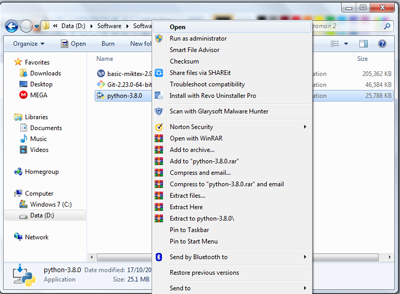
\includegraphics[width=4cm]{figures/1184030/variabel/1.png}
			\centering
			\caption{implementasi variabel}
			\end{figure}
		\end{enumerate}
	\item Kode Memasukkan Input dari User dan Menghasilkan Output ke Layar.\\
	\begin{enumerate}
	\item Input merupakan masukan yang diberikan kepada program. Dalam python, terdapat 2 sintaks fungsi yang digunakan untuk mengambil inputan. Di antaranya yaitu :
		\begin{enumerate}
		\item fungsi input()\\
		fungsi ini digunakan untuk mengambil inputan berupa data angka. Namun pada python 3, fungsi ini juga dapat digunakan untuk mengambil inputan berupa data huruf\
		\item fungsi input berupa raw input\\
		fungsi ini digunakan untuk mengambil inputan berupa data huruf. Fungsi inputan jenis ini hanya dapat digunakan pada python versi 2. Sedangkan pada python versi 3, semua fungsi input dapat digunakan pada fungsi input()
		\end{enumerate}
	\item Output merupakan hasil keluaran yang dihasilkan dari suatu program. Untuk menghasilkan keluaran yang dibuat oleh program, maka digunakan fungsi print() di dalam scipt program
	\end{enumerate} 
	\item Operator Dasar Matematika dan Mengubah Tipe Data\\
		\begin{itemize}
		\item dasar yang ada pada bahasa pemrograman python ada 6. Di antaranya yaitu :
		\begin{enumerate}
			\item Aritmatika\\
				Berikut ini merupakan operasi dasar aritmatika pada python :
				\begin{figure}[H]
				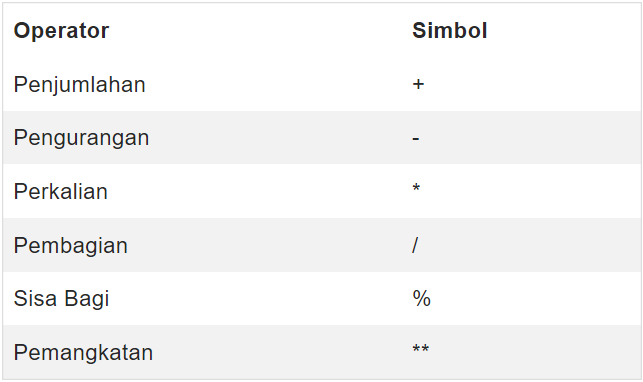
\includegraphics[width=4cm]{figures/1184030/arit.png}
				\centering
				\caption{operator aritmatika}
				\end{figure}
			\item Pembanding\\
				Berikut ini merupakan operasi pembanding pada python :
				\begin{figure}[H]
				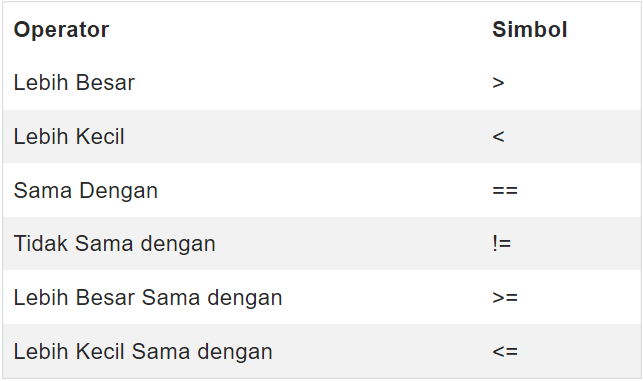
\includegraphics[width=4cm]{figures/1184030/pembanding.png}
				\centering
				\caption{operator pembanding}
				\end{figure}
			\item Penugasan\\
			Operator penugasan memiliki fungsi untuk memberi tugas kepada variabel.
				\begin{figure}[H]
				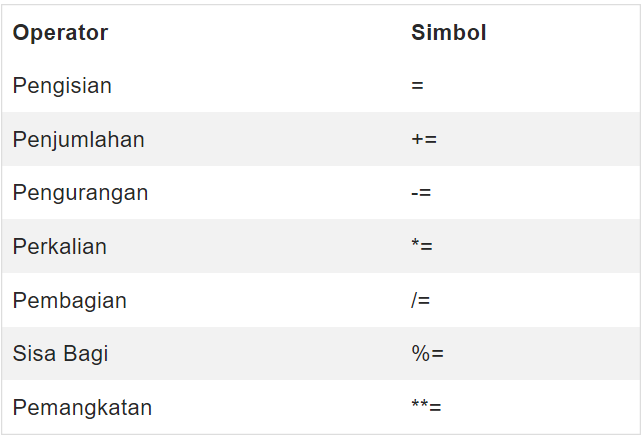
\includegraphics[width=4cm]{figures/1184030/penugasan.png}
				\centering
				\caption{operator pembanding}
				\end{figure}
			\item Logika\\
			Operator logika berfungsi untuk menjalankan operasi logika. Operasi logika terdiri atas or, and dan not. Berikut ini merupakan notasi yang merupakan operator logika
				\begin{figure}[H]
				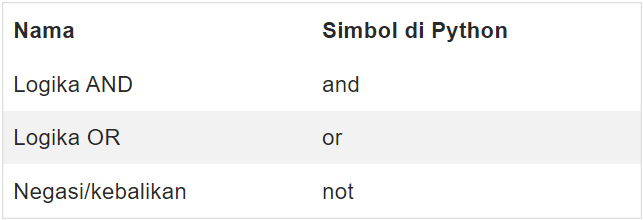
\includegraphics[width=4cm]{figures/1184030/logika.png}
				\centering
				\caption{operator logika}
				\end{figure}
			\item Bitwise\\
			Operasi ini merupakan operasi yang digunakan pada bilangan bit ataupun binary. Operasi bitwise meliputi :
				\begin{figure}[H]
				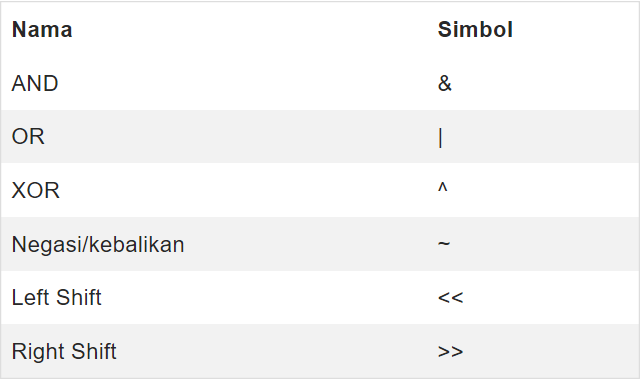
\includegraphics[width=4cm]{figures/1184030/bitwise.png}
				\centering
				\caption{operator bitwise}
				\end{figure}
			\item Ternary\\
			Operator ini disebut juga sebagai operator kondisi. Hal itu dikarenakan operator ini biasanya digunakan pada percabangan if else.
			\end{enumerate}
			\item Mengkonversi Tipe Data
				\begin{enumerate}
					\item Tipe data Integer
					\item Tipe data String
					\item Tipe data Float
					\item Tipe data Complex
				\end{enumerate}
				Untuk mengkonversi tipe data, kita hanya perlu untuk menambahkan tipe data yang akan kita konversikan menjadi. Contoh penamaannya :
				string = str(var) 
				float = float(var) 
				kompleks = complex(var) 
				long = long(var)\\
				keterangan : var merupakan variabel yang akan kita ubah tipe datanya.\\ 
		\end{itemize} 		
	\item Sintaks Perulangan
		\begin{enumerate}
			\item FOR\\
				For merupakan perulangan yang akan mengulang kondisi true sampai batas yang telah ditentukan. BErikut ini merupakan contoh penggunakan sintaks perulangan for.\\
				\begin{figure}[H]
				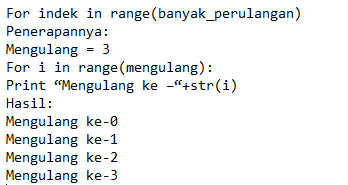
\includegraphics[width=4cm]{figures/1184030/for.png}
				\centering
				\caption{contoh penggunaan kondisi perulangan for}
				\end{figure}
			\item While\\
				While merupakan perulangan yang akan terjadi dengan dua kondisi jika benar dan jika salah. Berikut ini merupakan contoh penggunaan sintaks perulangan while.\\
				\begin{figure}[H]
				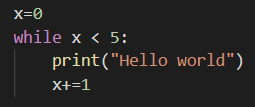
\includegraphics[width=4cm]{figures/1184030/while.png}
				\centering
				\caption{contoh penggunaan perulangan while}
				\end{figure}
		\end{enumerate}
	\item Sintaks Kondisi\\
		\begin{enumerate}
		\item Struktur if dengan kondisi tunggal.\\
			Struktur if dengan kondisi tunggal adalah suatu struktur yang memiliki suatu perlakuan jika terjadi suatu kondisi. Akan tetapi, tidak terjadi sesuatu yang lain aau terjadi apa-apa ketika berada di dalam luar kondisi tersebut.\\
			struktur if kondisi tunggal yaitu :\\
			if (kondisi):\\
				aksi\\
			contoh penggunaan struktur if itu sendiri di antaranya :
				\begin{figure}[H]
				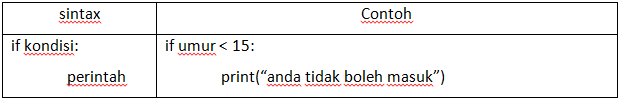
\includegraphics[width=4cm]{figures/1184030/if.png}
				\centering
				\caption{contoh penggunaan if kondisi tunggal}
				\end{figure}
		\item Struktur if else\\
		Struktur if else hampir sama dengan struktur if yang sebelumnya. Akan tetapi, pada struktur if else ini sendiri memiliki perbedaan dengan memiliki perlakuan terhadap 2 kondisi.\\
		struktur if else yaitu :\\
		if (kondisi):\\
			aksi\\
		else\\
			aksi2\\
		Berikut ini merupakan contoh pengaplikasiannya :\\
				\begin{figure}[H]
				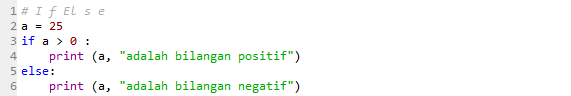
\includegraphics[width=4cm]{figures/1184030/ifelse.png}
				\centering
				\caption{contoh aplikasi struktur if else}
				\end{figure}
		\item Kondisi elif dan logika majemuk\\
		Kondisi if elif merupakan suatu strktur logika majemuk yang memiliki banyak pilihan aksi terhadap berbagai kemungkinan kejadian yang terjadi.\\
		Contoh pengaplikasian if elif yaitu :\\
				\begin{figure}[H]
				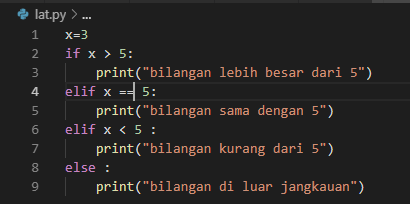
\includegraphics[width=4cm]{figures/1184030/ifelif.png}
				\centering
				\caption{penggunaan struktur if elif}
				\end{figure}
		\item Nested If atau if bersarang\\
		Nested if atau if bersarang, seperti namanya, ialah suatu struktur yang memiliki suatu keadian if di dalam suatu kejadian if yang lainnya.\\
		struktur penulisannya yaitu :\\
		if(kondisi):\\
			aksi\\
			if(kondisi):\\
			aksi\\
		berikut ini contoh pengaplikasian nested if :\\
				\begin{figure}[H]
				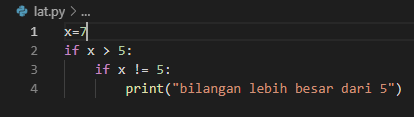
\includegraphics[width=4cm]{figures/1184030/ifsarang.png}
				\centering
				\caption{penggunaan struktur if sarang atau nested if}
				\end{figure}
		\end{enumerate}
	\item Jenis Error yang sering terjadi di Python
	\begin{enumerate}
	\item Logic Error.\\
	Logic error merupakan kesalahan yang terjadi karena kesalahan pembacaan data pada command perintah seperti data tidak terbaca atau tidak ada, dan tidak sesuai dengan aturannya.\\
	Contoh kesalahan tipe data yaitu :\\
	a='4'\\
	b=6\\
	print(a+b)\\
	\item Syntax Error\\
	Syntax error merupakan kesalahan yang disebabkan karena terjadinya kesalahan penulisan  baik format, command, karakter, ataupun simbol. Error yang disebabkan oleh kesalahan penulisan ini menyebabkan program yang telah dibuat tidak dapat berjalan dnegan baik. Contohnya pemberian titik dua atau colon (:) pada command if(kondisi):, for i in (range):\\
	\item Error Indentasi\\
	Error indentasi merupakan kesalahan yang terjadi karena spasi atau menjorok. Indentasi itu sendiri berasal dari bahasa inggris Indentation yang artinya menjorokkan. Indentasi biasanya digunakan di bahasa pemrograman lainnya untuk memperindah dan mempermudah pembacaan command perintah saja. Sedangkan pada bahasa pemrograman python, indentasi digunakan sebagai penanda blok program. Sehingga indentas pada python sangatlah penting karena jika dalam blok program tidak memiliki indentasi, maka program akan error dan tidak dapat dijalankan. Contoh errot indentasi yaitu pada penulisan printah if else sebagai berikut :\\
				\begin{figure}[H]
				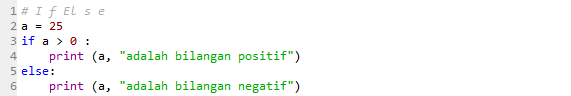
\includegraphics[width=4cm]{figures/1184030/ifelse.png}
				\centering
				\caption{penggunaan indentasi pada script}
				\end{figure}
	\end{enumerate}
	\item Try Except\\
	Try except merupakan penganganan error yang biasa terjadi ketika dalam penggunaan IO, database dan pengaksesan indeks suatu list atau dictionary.\\
				\begin{figure}[H]
				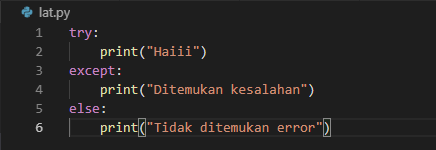
\includegraphics[width=4cm]{figures/1184030/tryex.png}
				\centering
				\caption{contoh penggunaan try except}
				\end{figure}
\end{itemize}
\section{KETERAMPILAN}
\lstinputlisting[language=Python]{src/NPM1.py}
\lstinputlisting[language=Python]{src/NPM2.py}
\lstinputlisting[language=Python]{src/NPM3.py}
\lstinputlisting[language=Python]{src/NPM4.py}
\lstinputlisting[language=Python]{src/NPM5.py}
\lstinputlisting[language=Python]{src/NPM6.py}
\lstinputlisting[language=Python]{src/NPM7.py}
\lstinputlisting[language=Python]{src/NPM8.py}
\lstinputlisting[language=Python]{src/NPM9.py}
\lstinputlisting[language=Python]{src/NPM10.py}
\lstinputlisting[language=Python]{src/NPM11.py}
\section{KETERAMPILAN PENANGANAN ERROR}
\begin{enumerate}
\item peringatan error pada praktek kedua dan penjelasan penanganan error tersebut.\\
Peringatan error yang muncul salah satunya yaitu seperti gambar di bawah ini :\\
				\begin{figure}[H]
				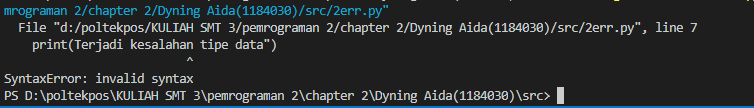
\includegraphics[width=10cm]{figures/1184030/penanganan.png}
				\centering
				\caption{peringatan error}
				\end{figure}
		Cara penanganan yang digunakan untuk mengatasi error tersebut yaitu dengan merujuk ke baris/line ke-7 dan kemudian mengecek sintaks yang salah ataupun tidak sesuai dengan aturan penulisan pada python. Pada sintaks tersebut ditemukan kesalahan pada penulisan print(Terjadi kesalahan tipe data"). Seharusnya, penulisan yang benar untuk mencetak string adalah dengan menyertakan dua tanda kutip di antara kata atau kalimat yang akan dicetak. Sehingga menjadi print("Terjadi kesalahan tipe data").
\item file 2err.py
\lstinputlisting[language=Python]{src/2err.py}
\end{enumerate}